 \documentclass{beamer}

\newlength{\wideitemsep}
\setlength{\wideitemsep}{\itemsep}
\addtolength{\wideitemsep}{10pt}
\let\olditem\item
\renewcommand{\item}{\setlength{\itemsep}{\wideitemsep}\olditem}

\usepackage[utf8]{inputenc}
\usepackage[russian]{babel}
\usepackage{cmap}

\mode<presentation> {
\usetheme{Madrid}
\setbeamertemplate{caption}[numbered]
}

\usepackage{graphicx} % Allows including images
\usepackage{booktabs} % Allows the use of \toprule, \midrule and \bottomrule in tables

\title[Технологии разработки ПО]{Kormushka:\\финансовый микроменеджмент}

\author{Black team.}
\institute[СПб ПУ]
{
Санкт-Петербургский государственный политехнический университет \\
\medskip
\textit{https://github.com/SemenMartynov/kormushka}
}
\date{\today}

\begin{document}

\begin{frame}
\titlepage
\end{frame}

\begin{frame}
\frametitle{Содержание}
\tableofcontents
\end{frame}

%------------------------------------------------
\section{Команда}
%------------------------------------------------

\begin{frame}
\frametitle{Команда: распределение ролей}

\begin{itemize}
\item Мяснов Александр (Client),
\bigskip
\bigskip
\item Дедков Сергей (Project Manager),
\medskip
\item Антон Абрамов (Lead programmer),
\medskip
\item Влад Бусаров (Software Engineer),
\medskip
\item Николай Патраков (Software Engineer),
\medskip
\item Семён Мартынов (Quality Assurance).
\end{itemize}

\end{frame}

%------------------------------------------------
\section{Задача}
%------------------------------------------------

\begin{frame}
\frametitle{О проекте}

\begin{figure}
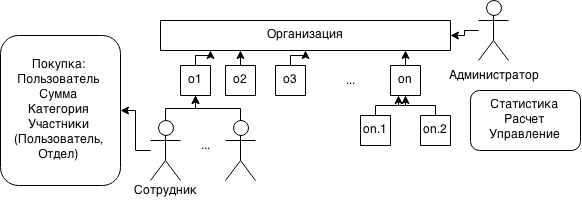
\includegraphics[scale=0.5]{res/r2_about}
\caption{Обзор проекта}
\end{figure}

\end{frame}

%------------------------------------------------

\begin{frame}
\frametitle{Цели проекта}

В процессе общения с заказчиком, вектор работ был несколько изменён:

\begin{itemize}
\item появилась интеграция с LDAP
\item исчез взаиморасчёт участников группы
\item появились отделы и лимиты
\item исчез внешний сервис (теперь мы работам в корпоративной сети)
\end{itemize}
\bigskip
Задача: ведение базы трат и формирование подробных отчётов.

\end{frame}

%------------------------------------------------
\section{Задачи первого спринта}
%------------------------------------------------

\begin{frame}
\frametitle{Список решенных задач}

На данный момент закрыто 33 задачи (в т.ч. отклонённые):
\begin{itemize}
\item Выявлены функциональные требования и проведёт анализ для выбора технологий
\item Разработана общая архитектура (но архитектура модулей требует доработки)
\item Реализована альфа-версия, реализующая функционал некоторых модулей (управление пользователями, добавление данных о тратах)
\item Реализовано взаимодействие с LDAP (пока в полном режиме, без ограничения прав)
\item Внедрена "культура комитов" (в master всё попадает через pull-request) и "культуры тасков" (правила открытия/закрытия и моток для задач)
\item Развернут сервер с демо-версией продукта (? нужен ли)
\end{itemize}


\end{frame}

%------------------------------------------------

\begin{frame}
\frametitle{Список решенных задач (продолжение)}

(...продолжение):
\begin{itemize}
\item Запущено (в тестовом режиме) использование Jenkins CI
\item Оформлена wiki со статьями по работе проекта
\item Развернут сервер с демо-версией продукта (? нужен ли)
\item bug fixing
\end{itemize}


\end{frame}

%------------------------------------------------

\begin{frame}
\frametitle{Список нерешенных задач}

На данный момент открыты 26 задач (в т.ч. мама-задачи, баги и research-задачи):
\begin{itemize}
\item Нет финальной согласованной версии ТЗ
\item Нет полного покрытия тестами
\item Нет модуля статистики
\item Не начата работа по созданию мобильного клиента
\end{itemize}


\end{frame}

%------------------------------------------------

\begin{frame}
\frametitle{Основные блоккеры}

Основные проблемы, с которыми мы встретились:
\begin{itemize}
\item Большой объём задач по текущему семестру (особенно защита информации).
\item Большой объем задач с предыдущего семестра.
\item Ощутимый порог вхождения (Django 1.7, WSGI, LDAP и даже некоторые моменты работы с git).
\item Библиотеки для работы с LDAP под Pyhton 3
\item Технические проблемы: у Влада сгорел винчестер.
\end{itemize}


\end{frame}

%------------------------------------------------
\section{Статистика использования СКВ}
%------------------------------------------------

\begin{frame}
\frametitle{Статистика использования СКВ}

\begin{figure}
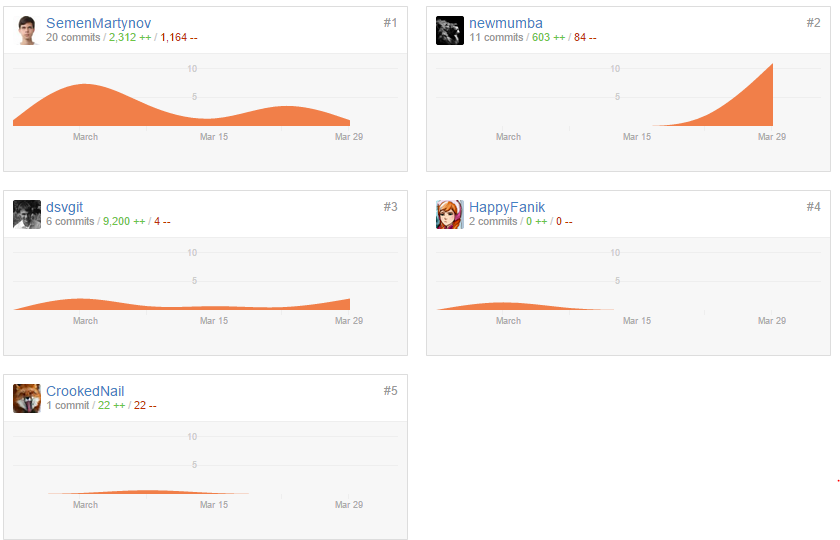
\includegraphics[scale=0.47]{res/r2_statistic}
\caption{Статистика коммитов с 22 февраля по 3 апреля, без учёта merge-коммитов и только по ветке master}
\end{figure}


\end{frame}

%------------------------------------------------
\section{Статистика использования СКВ}
%------------------------------------------------

\begin{frame}
\frametitle{Статистика использования СКВ}

\begin{figure}
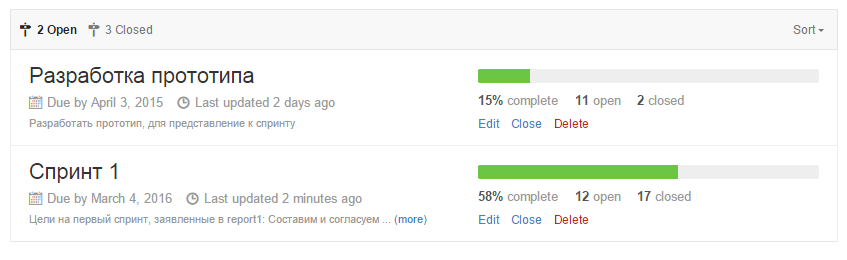
\includegraphics[scale=0.3]{res/r2_ms_open}
\caption{Opened milestones}
\end{figure}

\begin{figure}
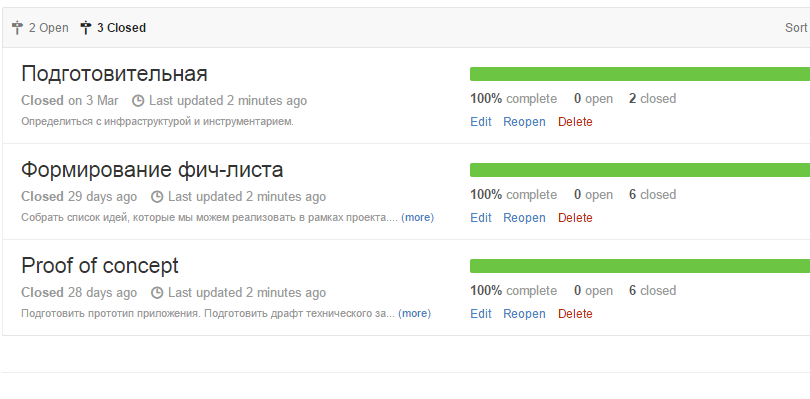
\includegraphics[scale=0.3]{res/r2_ms_closed}
\caption{Closed milestones}
\end{figure}

\end{frame}


%------------------------------------------------
\section{Общение с заказчиком}
%------------------------------------------------

\begin{frame}
\frametitle{Общение с заказчиком}

С заказчиком за время спринта было проведено три встречи.

Протоколы каждой встречи хранятся на wiki проекта.

\begin{itemize}
\item 10/III - заказчику было предложено 3 концепта (мобильное приложение с p2p обменом, внешний веб-сервис, плагин к RedMine). Был выбран промежуточный вариант между первым и вторым.
\item 17/III (Skype) - пересмотрен принцип групп, появилась идея интеграции с LDAP.
\item 23/III - общение в формате вопрос-ответ. Проведено уточнение множества важных деталей.
\end{itemize}

\end{frame}


%------------------------------------------------
\section{Тестирование}
%------------------------------------------------

\begin{frame}
\frametitle{Тестирование}

Используется Jenkins CI (ver. 1.607) и плагины:

\begin{itemize}
\item Cobertura Plugin (Покрытие кода).
\item Violations Plugin (Отчеты о коде — pylint, pyflakes, pep8).
\item GitHub API Plugin (получение кода из репозитория).
\end{itemize}


\begin{figure}
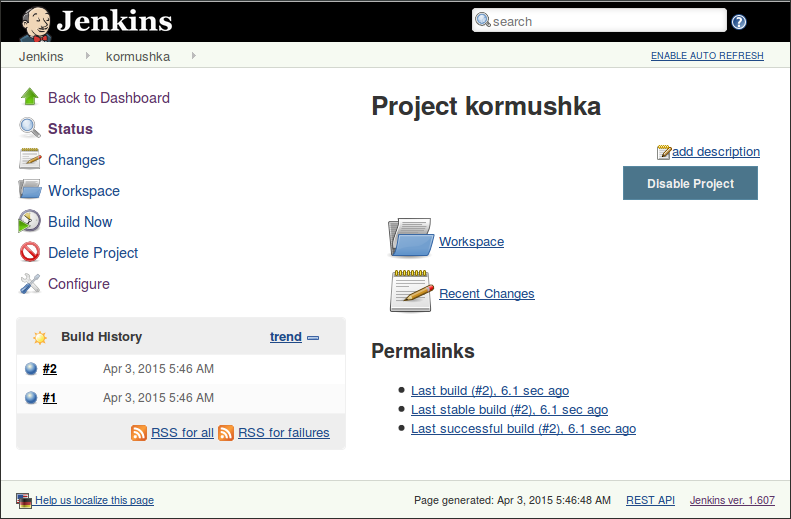
\includegraphics[scale=0.25]{res/r2_jenkins}
\caption{Jenkins - continuous integration}
\end{figure}

\end{frame}

%------------------------------------------------
\section{Документирование}
%------------------------------------------------

\begin{frame}
\frametitle{Документирование}

Планируется введение Doxygen.

На данный момент схемы (svg) и статьи в wiki.

\begin{figure}
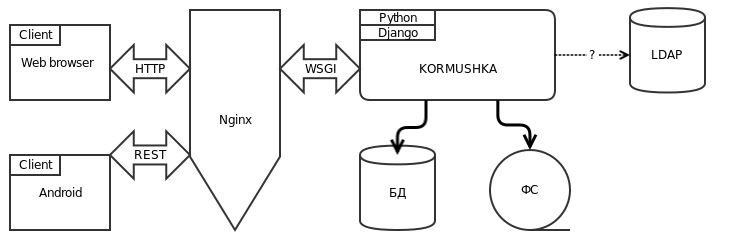
\includegraphics[scale=0.60]{res/r2_kormushka_ext}
\caption{Пример используемой схемы: внешняя архитектура}
\end{figure}


\end{frame}


%------------------------------------------------
\section{Демонстрация результатов}
%------------------------------------------------

\begin{frame}
\frametitle{Демонстрация достигнутых результатов}

\begin{figure}[h!]
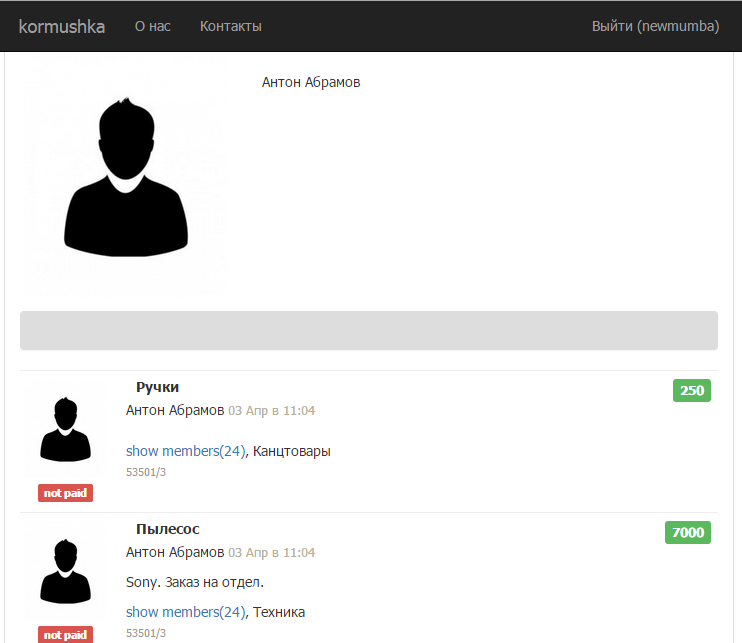
\includegraphics[scale=0.40]{res/r2_result}
\caption{Пример программы}
\end{figure}

\end{frame}

%------------------------------------------------
\section{Цели второго спринта}
%------------------------------------------------

\begin{frame}
\frametitle{План второго спринта}

К концу второго спринта мы достигнем следующих результатов:
\medskip
\begin{itemize}
\item Мобильный клиент (Android)
\item Построение красивых графиков статистики
\item Полное покрытие тестами
\item Автоматически генерируемая документация
\item Доработать архитектуру
\item Разработать alpha-версию
\end{itemize}

\end{frame}

%------------------------------------------------
\section{Вопросы}
%------------------------------------------------

\begin{frame}
\Huge{\centerline{Спасибо за внимание}}
\Huge{\centerline{Вопросы?}}
\end{frame}

%----------------------------------------------------------------------------------------

\end{document} 
